\graphicspath{{ch6_oct_localization/}{Figures/}}
% \graphicspath{{Figures/}}

\chapter{Predicting OCT biological marker localization from weak annotations}
\label{chapter:oct}

\sidechaptersummary{Localization of biological markers on ETDRS grid, Domain knowledge incorporation into a loss function, En-face biological marker segmentation}

\subsubsection{Synopsis}Recent developments in deep learning have shown success in accurately predicting the location of biological markers in Optical Coherence Tomography (OCT) volumes of patients with Age-Related Macular Degeneration (AMD) and Diabetic Retinopathy (DR). We propose a method that automatically locates biological markers to the Early Treatment Diabetic Retinopathy Study (ETDRS) rings, only requiring B-scan-level presence annotations. We trained a neural network using 22,723 OCT B-Scans of 460 eyes (433 patients) with AMD and DR, annotated with slice-level labels for Intraretinal Fluid (IRF) and Subretinal Fluid (SRF). The neural network outputs were mapped into the corresponding ETDRS rings. We incorporated the class annotations and domain knowledge into a loss function to constrain the output with biologically plausible solutions. The method was tested on a set of OCT volumes with 322 eyes (189 patients) with Diabetic Macular Edema, with slice-level SRF and IRF presence annotations for the ETDRS rings. Our method accurately predicted the presence of IRF and SRF in each ETDRS ring, outperforming previous baselines even in the most challenging scenarios. Our model was also successfully applied to en-face marker segmentation and showed consistency within C-scans, despite not incorporating volume information in the training process. We achieved a correlation coefficient of 0.946 for the prediction of the IRF area. 

\subsubsection{Publication}This chapter is based on a publication\sideauthorcite{tejero2023predicting}, and its contents have been modified slightly to be more consistent with the rest of the thesis. More specifically, \Cref{tab:var_list_loc} has been added to the main text from the supplementary material.

\subsubsection{Author contributions}The work in this chapter was done in collaboration with the University Hospital Bern. The contributing authors were Pablo Márquez Neila, Thomas Kurmann, Mathias Gallardo, Martin Zinkernagel, Sebastian Wolf, and Raphael Sznitman. My contribution was the co-development and implementation of the method; conception and evaluation of the experiments and, together with the co-authors, writing of the paper.


\section{Introduction}
\label{sec:full_weakintro}
Semantic segmentation is a fundamental computer vision task with applications in numerous domains such as autonomous driving~\sidecite{cordts2016cityscapes,siam2017deep}, scene understanding~\sidecite{sless2019road}, surveillance~\sidecite{tseng2021person} and medical diagnosis~\sidecite{chen2020deep,hesamian2019deep}. As the advent of deep learning has significantly advanced the state-of-the-art, many new application areas have come to light and continue to do so too. This growth has brought and continues to bring exciting domain-specific datasets for segmentation tasks~\sidecite{islam2020semantic,li2020mas3k,Bodenstedt2018,liu2020fsd,WelinderEtal2010}. 

Today, the process of establishing machine learning-based segmentation models for any new application is relatively well understood and standard. Only once an image dataset is gathered and curated, can machine learning models be trained and validated. In contrast, building appropriate datasets is known to be difficult, time-consuming, and yet paramount. Beyond the fact that collecting images can be tedious, a far more challenging task is producing ground-truth segmentation annotations to subsequently train (semi) supervised machine learning models. This is mainly because producing segmentation annotations often remains a manual task. As reported in~\sidecite{Bearman16}, generating segmentation annotations for a single PASCAL image~\sidecite{pascal-voc-2012} takes over 200 seconds on average. This implies over 250 hours of annotation time for a dataset containing a modest 5'000 images. What often further exacerbates the problem for domain-specific datasets is that only the dataset designer, or a small group of individuals, have enough expertise to produce the annotations (\eg, doctors, experts, etc.), making crowd-sourcing ill-suited. 
%\begin{figure*}[t]
%\centering
%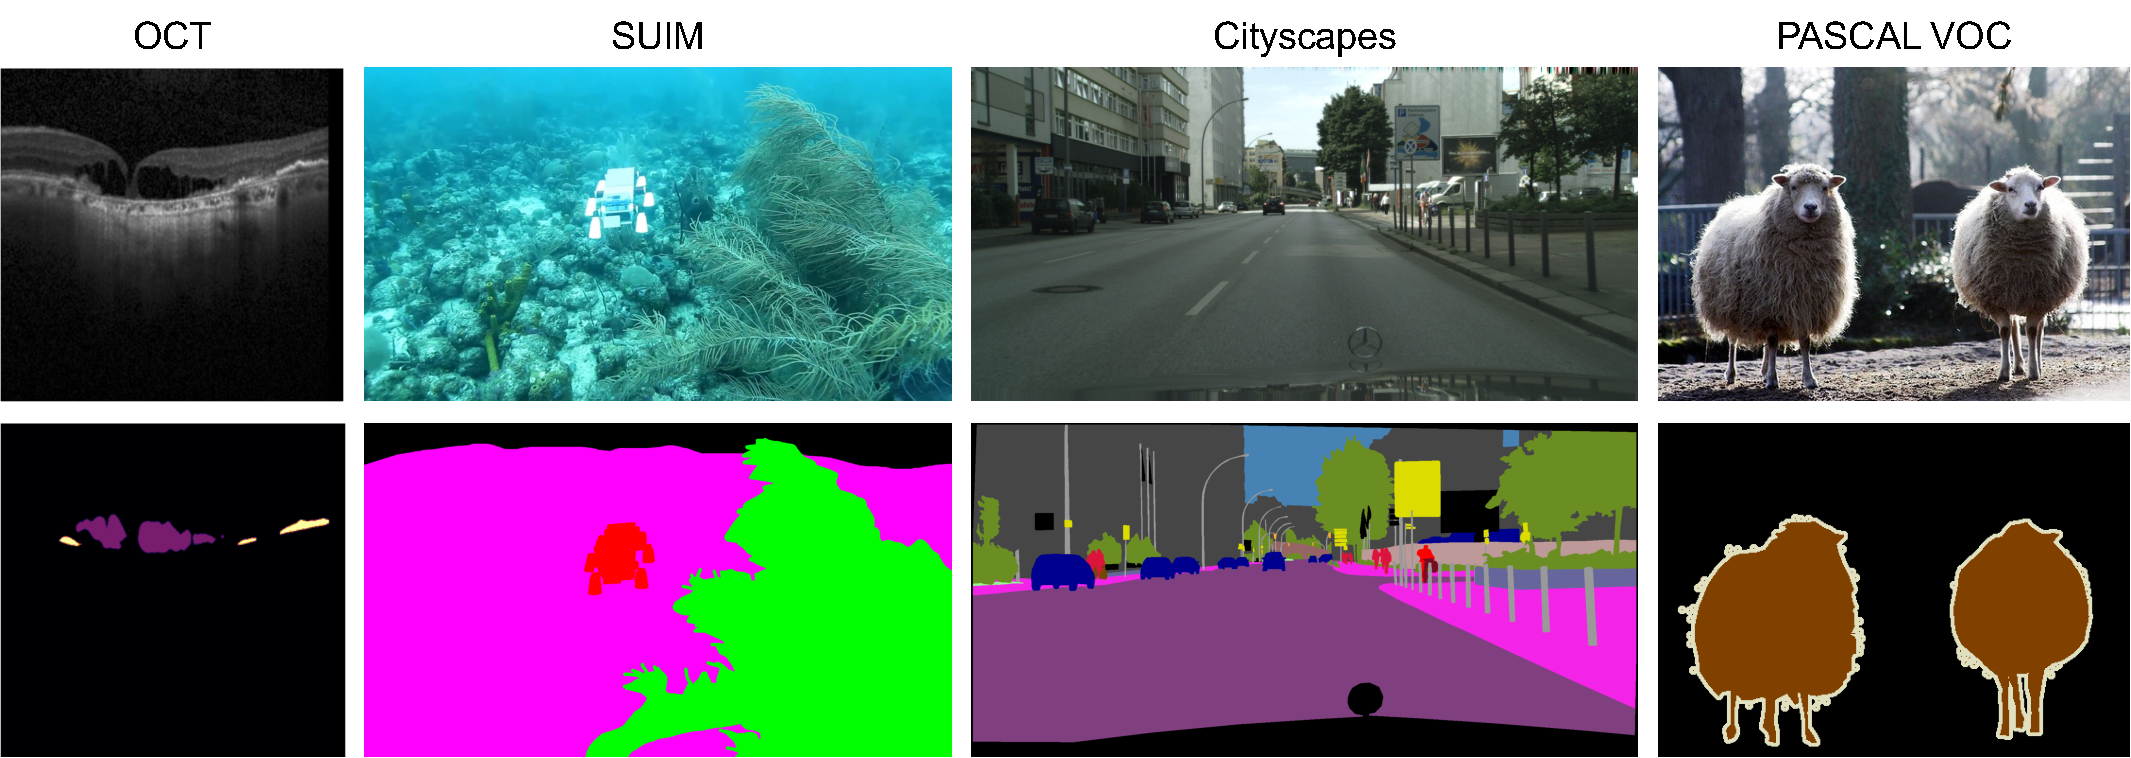
\includegraphics[width=0.99\textwidth]{Figures/datasets.pdf}
%\caption{Illustration of different semantic segmentation applications; OCT: Pathologies of the eye in OCT images, SUIM: Underwater scene segmentation~\sidecite{islam2020semantic}, Cityscape: street level scene segmentation~\sidecite{cordts2016cityscapes}, PASCAL VOC: natural object segmentation.}
%\label{fig:datasets}
%\end{figure*}

\plainwidefig[t]{1}{Figures/datasets.pdf}{Illustration of different semantic segmentation applications; OCT: Pathologies of the eye in OCT images, SUIM: Underwater scene segmentation~\cite{islam2020semantic}, Cityscape: street level scene segmentation~\cite{cordts2016cityscapes}, PASCAL VOC: natural object segmentation.}{fig:fullweak_datasets}

To overcome this challenge, different paradigms have been suggested over the years. Approaches such as Active Learning~\sidecite{Cai21,Casanova2020Reinforced,Konyushkova15} aim to iteratively identify subsets of images to annotate so as to yield highly performing models. Transfer learning has also proved to be an important tool in reducing annotation tasks~\sidecite{Ding2019,heker2020joint,kolesnikov2020big,koleshnikov2021,Liang2020,menegola2017}. For instance, \sidecite{Mensink}~show that training segmentation models from scratch is often inferior to using pre-training models derived from large image classification datasets, even when the target application domain differs from the source domain. Finally, weakly-supervised methods~\sidecite{ahn2018learning,Papandreou15} combine pixel-wise annotations with other weak annotations that are faster to acquire, thereby reducing the annotation burden. In particular, Papandreou~\etal~\sidecite{Papandreou15} showed that combinations of strong and weak annotations (\eg, bounding boxes, keypoints, or image-level tags) delivered competitive results with a reduced annotation effort. In this work, we rely on these observations and focus on the weakly supervised segmentation setting.


In the frame of designing annotation campaigns, weakly-supervised approaches present opportunities for efficiency as well. Instead of completely spending a budget on a few expensive annotations, weakly-supervised methods allow a proportion of the budget to be allocated to inexpensive, or weak, labels. That is, one could spend the entire annotation budget to manually segment available images, but would ultimately lead to relatively few annotations. Conversely, weak annotations such as image-level labels are roughly 100~times cheaper to gather than their segmentation counterparts~\sidecite{Bearman16}. Thus, a greater number of weakly-annotated images could be used to train segmentation models at an equal cost. In fact, under a fixed budget, allocating a proportion of the budget to inexpensive image-level class labels has been shown to yield superior performance compared to entirely allocating a budget to segmentation labels~\sidecite{Bearman16}.

Yet, allocating how an annotation budget should be distributed among strong and weak annotations is challenging, and inappropriate allocations may severely impact the quality of the final segmentation model. For example, spending the entire budget on image-level annotations will clearly hurt the performance of a subsequent segmentation model. Instead, a naive solution would be to segment and classify a fixed proportion of each \sidenote{\eg, 80\% of the budget allocated for segmentation annotations and 20\% for classification.}. Knowing what proportion to use for a given dataset is unclear, however. Beyond this, there is no reason why the same fixed proportion would be appropriate across different datasets or application domains. That is, it would be highly unlikely that the datasets shown in \cref{fig:fullweak_datasets} all require the same proportion of strong and weak annotations to yield optimal segmentation models.

Despite its importance, choosing the best proportion of annotation types remains a largely unexplored research question. Weakly-supervised and transfer-learning methods generally assume that the annotation campaign and the model training are independent and that all annotations are simply available at training time. While active learning methods do alternate between annotation and training, they focus on choosing optimal samples to annotate rather than choosing the right type of annotations. Moreover, most active learning methods ignore constraints imposed by an annotation budget. More notable, however, are the recent works of Mahmood {\it et.~al.}~\sidecite{mahmood2022, mahmood2022optimizing} which aim to determine what weak and strong annotation strategy is necessary to achieve a target performance level. While noteworthy, this objective differs from that here, whereby given a fixed budget, what strategy is best suited for a given new dataset?

To this end, we propose a novel method to find an optimal budget allocation strategy in an online manner\sidedef{online learning}{The data is accessible in a sequential order and is employed to update the model at each step.}. Using a collection of unlabeled images and a maximum budget, our approach selects strong and weak annotations, constrained by a given budget, that maximize the performance of the subsequent trained segmentation model. To do this, our method iteratively alternates between partial budget allocations, label acquisition, and model training. At each step, we use the annotations performed so far to train multiple models to estimate how different proportions of weak and strong annotations affect model performance. A Gaussian Process models these results and maps the number of weak and strong annotations to the expected model improvement. Computing the Pareto optima between expected improvement and costs, we choose a new sub-budget installment and its associated allocation so to yield the maximum expected improvement. We show in our experiments that our approach is beneficial for a broad range of datasets, and illustrate that our dynamic strategy allows for high performances, close to optimal fixed strategies that cannot be determined beforehand.

\section{Methods}
\label{sec:oct_method}
Our objective is to train a method capable of inferring in which ETDRS ring different markers are located, but only using 2D OCT slices and associated slice-level binary annotations. In a 2D OCT slice, ETDRS rings correspond to a set of non-continuous vertical stripes (see~\Cref{fig:etdrs_rings}). From the placement of the ETDRS rings on the OCT volume, we make the following three important observations: (1) depending on where an OCT slice is positioned in the volume, different ETDRS rings are visible in the slice, (2) the width of different rings depends on where an OCT slice is positioned and (3) ring symmetry is preserved regardless of the slice position. We will explicitly leverage these observations to design and train our approach.

%\begin{figure}[]
%\centering
%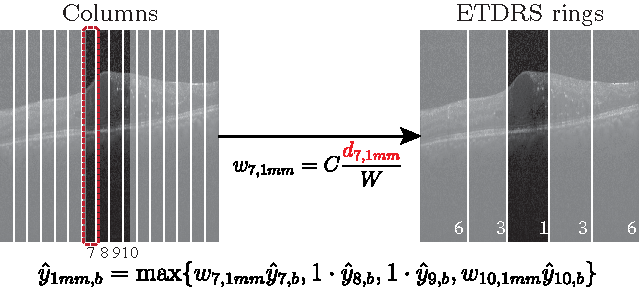
\includegraphics[width=.8\textwidth]{Figures/columns.pdf}
%\caption{Mapping column predictions to ring predictions for the central slice of an OCT~volume. The column layout (left) is shared among all slice positions. The ring layout (right) is specific to the slice location in the volume. $w_{i,j}$ is the contribution of ring $j$ in the $i$-th column and $\haty_{i,b}$ is the prediction for ring $i$ and marker $b$.
%}
%\label{fig:columns}
%\end{figure}

\textfig[t]{1}{Figures/columns.pdf}{Mapping column predictions to ring predictions for the central slice of an OCT~volume. The column layout (left) is shared among all slice positions. The ring layout (right) is specific to the slice location in the volume. $w_{i,j}$ is the contribution of ring $j$ in the $i$-th column and $\haty_{i,b}$ is the prediction for ring $i$ and marker $b$.}{fig:columns}

Specifically, instead of training our method to produce different outputs depending on the slice location, we predefined a partition of 2D OCT slices into image columns\sidenote{See \Cref{fig:columns}, left.}. That is, we will train our method to produce predictions for each of these columns, regardless of the specific slice location within the volume. At the end of this section we describe the straightforward post-processing mapping from column-level predictions to the ETDRS rings (as shown in \Cref{fig:columns} left).


\subsection{Model}

\begin{margintable}[]\small
\caption{List of variables and their description}
\label{tab:var_list_loc}
\begin{tabular}{@{}cl@{}}
\toprule
\textbf{Var.}       & \textbf{Description}                                                                                         \\ \midrule
$H$            & Slice height                                                                              \\
$W$            & Slice width                                                                           \\
$C$            & Num. of columns                                              \\
$\x$           & 2D OCT slice                                                                                        \\
$\x'$          & Flipped OCT slice                                                                                \\
$\haty$        & Probs. for $\x$                                                \\
$\haty'$       & Probs. for $\x'$                                   \\
$\haty_{0,b}$  & Prob. of~$b$ in the slice                                              \\
$\haty_{c, b}$ & Prob. of~$b$ in column~$c$                                                        \\
$\y_0$         & Slice-level annotations                                                                             \\
$\y_{0,b}$     & Annotations for $b$                                                           \\
$\z$           & Feature map                                                                      \\
$\d_0$         & OCT slice descriptor               \\
$\d_c$         & Column~$c$ descriptor    \\ \bottomrule
\end{tabular}
\end{margintable}

Formally, we partition a 2D OCT slice,~$\x$, into $C$ equally spaced columns. We wish to train a model~$f:[0,1]^{H\times W} \to [0,1]^{(1+C)\times B}$ that maps $\x$ to a collection of probabilities~$\haty$, where $B$~is the number of different possible types of markers to be found. For each marker~$b\in B$, the collection~$\haty$ contains both the probability of presence of~$b$ in the entire OCT slice,~$\haty_{0,b}$, and the probability of presence of~$b$ in each column~$c\in C$, denoted~$\haty_{c, b}$. Our training data is made of tuples~$(\x, \y_0)$, with OCT slice~$\x$ and corresponding slice-level annotations~$\y_0\in\{0, 1\}^B$ with no reference whatsoever to the ring or column in which they are located.
%\begin{figure}[t]
%\centering
%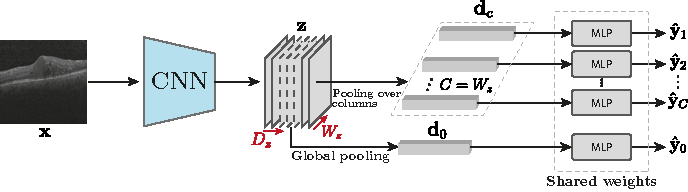
\includegraphics[width=\textwidth]{Figures/architecture.pdf}
%\caption{Our proposed network architecture: usage of partial pooling to extract information from the feature map to infer location outputs with a set of shared-weight MLPs.}
%\label{fig:architecture}
%\end{figure}

\widefig[t]{1}{Figures/architecture.pdf}{Proposed network architecture: usage of partial pooling to extract information from the feature map to infer location outputs with a set of shared-weight MLPs.}{fig:architecture}

\Cref{fig:architecture} depicts our model architecture. The input OCT slice is processed by a CNN which produces a feature map~$\z \in \real^{D_z\times H_z\times W_z}$ with width equal to the number of columns~$C = W_z$. We then apply a number of pooling operations over the feature map~$\z$ to describe the entire OCT slice as well as every column~$c$. In particular, to identify markers that may appear as large or small in a given image, we set the descriptor of the entire OCT slice to be a $2D_z$-dimensional vector~$\d_0=[\avgpool(\z), \maxpool(\z)]$ obtained as the concatenation of average pooling and maximum pooling over the spatial dimensions of~$\z$. Likewise, the descriptor of every column~$c$ is another $2D_z$-dimensional vector~$\d_c=[\avgpool(\z_{\cdot,\cdot,c}), \maxpool(\z_{\cdot,\cdot,c})]$ obtained as the concatenation of the two pooling operators acting on the corresponding column of~$\z$. The descriptor vectors are then processed by a multi-layer perceptron (MLP) followed by an element-wise sigmoid activation to produce the final probabilities,
\begin{equation}
    \haty_0 = \sigma\left(\textrm{MLP}(\d_0)\right),\quad \quad 
    \haty_c = \sigma\left(\textrm{MLP}(\d_c)\right) \quad \forall c.
\end{equation}



\subsection{Training}

We use a combination of three loss terms to train our model. The first term uses the standard \autoindex{binary cross entropy} (BCE) of the slice-level predictions~$\haty_0$ with the slice-level ground-truth annotations~$\y_0$,
\begin{equation}
    \ell_1(\haty, \y_0) = \sum_{b} \textrm{BCE}(\haty_{0,b}, \y_{0,b}).
    \label{eq:l1}
\end{equation}

The second term incorporates constraints on column-level predictions based on the image-level ground-truth. Specifically, when a biological marker is not present in the input image, $\y_{0,b} = 0$, we penalize high predicted probabilities for~$b$ in all the columns. On the other hand, if the marker is present, $\y_{0,b}=1$, we encourage a high probability for~$b$ for at least one column. Formally, we compute,
\begin{equation}
    \ell_2(\haty, \y_{0,b}) = -\sum_b (1-\y_{0,b})\dfrac{1}{C}\sum_c \log (1-\haty_{c,b}) - \sum_b \y_{0,b}\max_c \log \haty_{c,b}.
    \label{eq:l2}
\end{equation}
The last term imposes invariance to horizontal symmetry on the column-level probabilities. When our model receives a horizontally flipped image~$\x'$, the predicted column-level probabilities~$\haty'$ should also be flipped, and therefore $\haty_{c,b}$~should be equal to~$\haty'_{C-c,b}$ for all~$b$. To this end, we penalize a symmetric KL~divergence\index{KL divergence} between the corresponding probabilities,
\begin{equation}
    \ell_3(\haty, \haty') = \dfrac{1}{2}\sum_{c, b} 
        \left(
            \infdiv{\haty_{c, b}}{{\haty'_{C-c, b}}} +
            \infdiv{\haty'_{c, b}}{{\haty_{C-c, b}}}
        \right).
\end{equation}

Specifically, $\ell_3$ incorporates the symmetry of the ETDRS rings we wish to induce in our model\sidenote{The addition of $\ell_3$ doubles the effective size of the training dataset and of the batches. However, this does not hurt performance as long as the new batches fit in GPU memory.}. Note that the desired horizontal symmetry cannot be obtained by random horizontal image flipping augmentation, however, as $\ell_3$ enforces predictions on the columns to be consistent regardless of whether the image is flipped or not.
Using a similar symmetry argument for $\ell_1$ and~$\ell_2$, our final loss is,
\begin{equation}
\label{eq:combinedLoss}
    \mathcal{L}(\haty, \haty', \y_0) =
        \ell_1(\haty, \y_0) + \ell_1(\haty', \y_0) + \ell_2(\haty, \y_0) + \ell_2(\haty', \y_0) + \ell_3(\haty, \haty'),
\end{equation}
where $\haty$~ and $\haty'$ are the predicted probabilities for the input image~$\x$ and corresponding horizontally-flipped version~$\x'$, respectively. \Cref{fig:loss_drawing} shows a graphical explanation for $\ell_2$ and $\ell_3$.
%\begin{figure}[t]
%\centering
%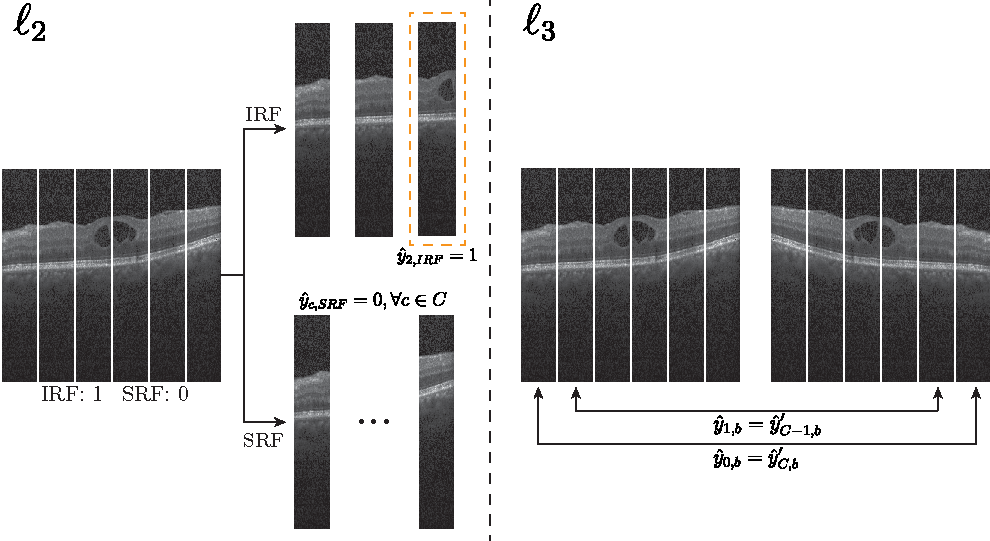
\includegraphics[width=0.85\textwidth]{Figures/loss_drawing.pdf}
%\caption{Graphical explanation for $\ell_2$ and $\ell_3$ in a slice where IRF is present and SRF is not. In this example, with $\ell_2$, we enforce that IRF must be present in at least one column while SRF is not found anywhere. With $\ell_3$ we incorporate symmetry consistency among the flipped and the non-flipped slices.}
%\label{fig:loss_drawing}
%\end{figure}

\textfig{1}{Figures/loss_drawing.pdf}{Graphical explanation for $\ell_2$ and $\ell_3$ in a slice where IRF is present and SRF is not. In this example, with $\ell_2$, we enforce that IRF must be present in at least one column while SRF is not found anywhere. With $\ell_3$ we incorporate symmetry consistency among the flipped and the non-flipped slices.}{fig:loss_drawing}


\subsection{Inference}
At test time, we can infer the layout of ETDRS rings in an OCT slice once a slice is evaluated by our network. This correspondence is not one-to-one, as a single ring usually contains several columns, and one column may be shared between two rings. To thus produce ring-level predictions, we compute the maximum of the probabilities of the columns contained in each ring. For columns spanning two rings, we weigh the contribution of the column by the proportion of the column inside each ring, as shown in \Cref{fig:columns}.

\section{Results}
\label{sec:oct_results}
We present the descriptive statistics of the training and testing sets in \Cref{tab:dataset}. The OCT data comes from the Dept. of Ophthalmology, Bern University Hospital (Switzerland) and was acquired using the Heidelberg Spectralis system. The resolution of all slices is 496×512 pixels. The training and testing sets are similar in terms of pathologies, with the main difference being  the granularity of the annotations: the training dataset only contains slice-level annotations for two biological markers, while the testing dataset includes additional ETDRS rings information at 1mm, 3mm and 6mm per slice. In addition, a subset of the testing dataset has been manually segmented. Therefore, pixel-wise annotations for IRF and SRF are also available in 54 volumes (2’646 OCT slices). None of the patients in this test data are present in the training data. The distribution of IRF and SRF occurrences in the testing dataset is given in \Cref{tab:results}.

\noindent
\begin{table*}[t]
\centering
\caption{Dataset description}
\label{tab:dataset}
\begin{tabular}{p{4cm}p{5.5cm}p{5.5cm}}
\toprule
 & Training dataset & Testing dataset \\ \midrule
Number of patients & 433 & 189 \\
Number of eyes & 460 & 322 \\
Number of slices & 22’723 & 28'322 \\
Present pathologies & Diabetic retinopathy with and without Diabetic Macular Edema (DME), and early, intermediate, and late AMD & DME \\
Annotations & Slice-level annotations for IRF and SRF & Slice-level SRF and IRF presence   annotations for the ETDRS rings at 1mm, 3mm, and 6mm \\ \bottomrule
\end{tabular}

\end{table*}

\subsection{Implementation and baselines}
The backbone model of our method is an EfficientNet-b4~\sideauthorcite{Tan2019} with ImageNet-initialized weights. As a preliminary step, we train the network alone in the task of IRF and SRF multilabel classification to produce slice-level predictions, and then fine-tune the entire model as described in the Methods section with the loss function of Eq. 5. We use a batch size of 32 slices\sidenote{A batch size of 32 means that we are using 32 slices and their flipped version for $\ell_3$.}, SGD with momentum of 0.9 and a base learning rate of $5\cdot10^{-3}$ which is scaled by 0.99 after every epoch. The feature map z of EfficientNet-b4 is sized 1792×16×16. We perform maximum and average pooling per column to produce C=16 descriptor vectors $d_c$ of dimension $2D_z=3584$, which are subsequently processed by the MLP to get 16 column-level predictions. The MLP itself consists of a single linear layer with 2 outputs for SRF and IRF, followed by a sigmoid activation. The column-level predictions are then mapped to ring-level predictions as explained at the end of the Methods section.

While there are no direct existing baselines for localization of OCT biological markers with weak annotations, we compare our method to the following alternative baselines:
\begin{itemize}
    \item \textbf{Masking} At test time, we mask the slice regions to only reveal relevant ETDRS rings and feed this to an EfficientNet trained on the slice-level detection task (as above). This masking has been done by replacing all pixels in the region to 0.
    
    \item \textbf{Masking with partial convolutions (PartConvs)} As in the \textbf{Masking} baseline but replacing all convolutional layers by partial convolutions~\sideauthorcite{Liuc}, except for those in the squeeze and excitation blocks~\sideauthorcite{Hu2019}, so to ignore masked regions.
    
    \item \textbf{Grad-CAM} We use Grad-CAM~\sideauthorcite{Selvaraju2019} to build a 16×16 heatmap for each output variable and pick the maximum value of each column. This serves as a column-level measurement of the presence of SRF and IRF. We use the pre-trained EfficientNet to obtain the final ring-level predictions by applying the same post-processing mapping explained at the end of the Methods section.

    \item \textbf{MS-CAM}~\sideauthorcite{ma2020} this approach consists of two stages: first, the activations of the different features of the resolutions are combined with Grad-CAM++~\sideauthorcite{chattopadhay2018grad} to obtain a pixel-wise segmentation. Second, these segmentations are refined using Conditional Random Fields on the \textit{en face} projection image\sidedef{\textit{En face} Projection}{Projection of the OCT metrics into the fundus, creating a top-down view.}. We reproduced the first stage and converted the resulting pixel-wise segmentation into rings. 
\end{itemize}

All methods were implemented using PyTorch. Our method and the baselines were trained for 10 epochs.

\subsection{Localization results}
\marginfig{Figures/example_columns.pdf}{Outputs of our method and baselines. We show the slice number (bottom right) and in which ring the marker can be found (top row). Incorrect detections are highlighted in red.}{fig:examples}

\Cref{tab:results} reports the performance of all methods in terms of AUC ROC and Average Precision (AP). Our method achieves the highest ROC-AUC and AP for every marker and ETDRS ring. The improvement is particularly notable for 6mm SRF, where our method doubles the performance of other baselines in AP. \Cref{fig:results_curves} compares our method's ROC and Precision-Recall curves and the PartConvs baseline throughout the three ETDRS rings. \Cref{tab:results} also shows the occurrence of both biological markers in each one of the rings. IRF is present in 51.5\% of the images in the testing set, while SRF is scarcer and present in only 2.8\%. This imbalance is further exacerbated in the ring annotations: as depicted in Figure 1, where the 6mm ring is present in all the B-Scans. However, 38.4\% have IRF in the 6mm ring, but only 0.4\% have SRF. This is explained by the fact that SRF is unlikely to be found in the outer rings, leading to a lower number of occurrences in the test set than IRF. 

\noindent
\begin{table*}[t]
\centering
\caption{Comparison of the proposed method to evaluated baselines in terms of AUC ROC and AP on the {\bf Location dataset} for all markers on the entire slice and in the different ETDRS rings. The first row indicates the occurrences of each marker in this dataset.\label{tab:results}}
\begin{tabular}{@{}TrSSSSSS|SS@{}}
\cmidrule(l){3-10}
\multicolumn{1}{l}{}          & \multicolumn{1}{l}{}           & \multicolumn{2}{c}{\textbf{1mm}} & \multicolumn{2}{c}{\textbf{3mm}} & \multicolumn{2}{c}{\textbf{6mm}}                   & \multicolumn{2}{c}{\textbf{Present}} \\ \cmidrule(l){3-10} 
\multicolumn{1}{l}{}          & \multicolumn{1}{l}{}           & \textbf{IRF}    & \textbf{SRF}   & \textbf{IRF}    & \textbf{SRF}   & \textbf{IRF}  & \multicolumn{1}{c|}{\textbf{SRF}}  & \textbf{IRF}      & \textbf{SRF}     \\ \midrule
\multicolumn{1}{l}{}          & \multicolumn{1}{r|}{Occ. (\%)} & 13.0            & 2.1            & 31.9            & 1.2            & 38.4          & \multicolumn{1}{c|}{0.4}           & 51.5              & 2.8              \\ \midrule
\multirow{4}{*}{\textbf{AUC}} & \multicolumn{1}{r|}{Masking}   & 92.6            & 91.7           & 89.6            & 81.6           & 92.7          & \multicolumn{1}{c|}{66.7}          & 96.5              & 96.2             \\
& \multicolumn{1}{r|}{PartConvs}    & \textbf{93.2}   & 94.1           & 90.2            & 89.8           & 91.7          & \multicolumn{1}{c|}{74.9}          & 94.2              & 89.7             \\
& \multicolumn{1}{r|}{Grad-CAM}  & 85.2            & 87.3           & 89.2            & 76.0           & 89.4          & \multicolumn{1}{c|}{64.6}          & 96.5              & 96.2             \\
& \multicolumn{1}{r|}{MS-CAM~\cite{ma2020}}  & 55.7            & 70.4           & 57.5            & 64.1           & 55.0          & \multicolumn{1}{c|}{56.0}           & 56.0              & 53.7            \\
& \multicolumn{1}{r|}{\bf{Ours}}  & 90.6            & \textbf{97.5}  & \textbf{92.7}   & \textbf{93.8}  & \textbf{94.1} & \multicolumn{1}{c|}{\textbf{95.1}} & \textbf{97.2}     & \textbf{97.7}    \\ \midrule
\multirow{4}{*}{\textbf{AP}}  & \multicolumn{1}{r|}{Masking}   & 76.9            & 48.3           & 84.2            & 17.2           & \textbf{88.5} & \multicolumn{1}{c|}{5.6}           & 96.1              & 72.3             \\
& \multicolumn{1}{r|}{PartConvs}    & 81.8            & 60.5           & 85.2            & 21.4           & 88.1          & \multicolumn{1}{c|}{8.2}           & 94.2              & 38.5             \\
& \multicolumn{1}{r|}{Grad-CAM}  & 88.2            & 68.4           & 86.9            & 25.4           & 78.7          & \multicolumn{1}{c|}{7.4}           & 96.1              & 72.3             \\

& \multicolumn{1}{r|}{MS-CAM~\cite{ma2020}}  & 70.3            & 38.5           & 64.1            & 14.4           & 54.3          & \multicolumn{1}{c|}{1.6}           & 55.6              & 3.1             \\

& \multicolumn{1}{r|}{\bf Ours}  & \textbf{92.1}   & \textbf{86.6}  & \textbf{93.7}   & \textbf{52.7}  & 88.3          & \multicolumn{1}{c|}{\textbf{19.1}} & \textbf{96.8}     & \textbf{77.9}    \\ \bottomrule
\end{tabular}
%\caption{Comparison of the proposed method to evaluated baselines in terms of AUC ROC and AP on the {\bf Location dataset} for all markers on the entire slice and in the different ETDRS rings. The first row indicates the occurrences of each marker in this dataset.
%\label{tab:results}
\end{table*}

\textfig[t]{1}{Figures/all_plots.pdf}{ROC and Precision-Recall curves for both markers and rings with our proposed method on the testing dataset (solid lines). Results are compared to Partial Convolutions (dashed lines) on the same dataset.
}{fig:results_curves}

\Cref{fig:examples} illustrates the performance of the different methods in several cases. We provide additional cases in \Cref{fig:app_oct_examples} in the Appendix.

%\begin{figure}[t]
%\centering
%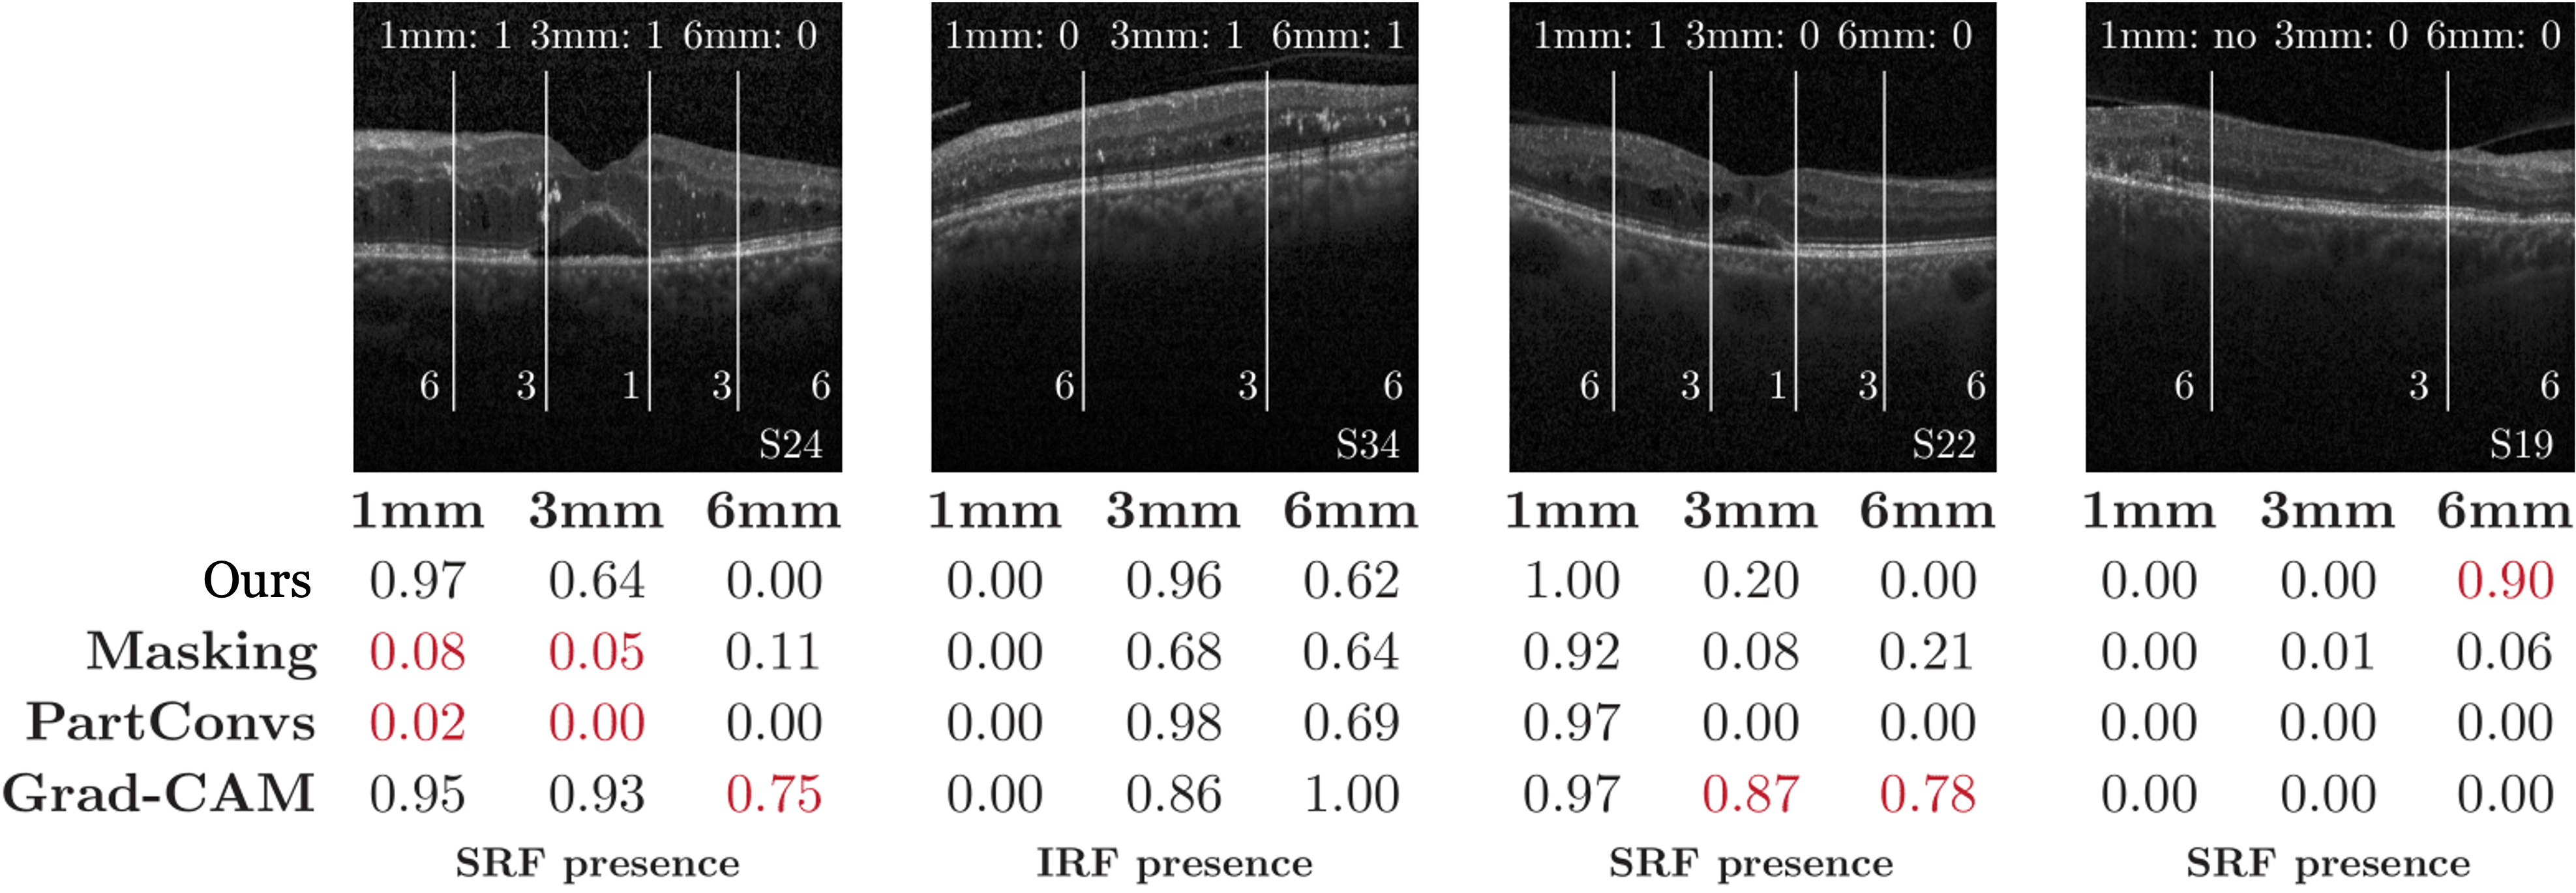
\includegraphics[width=.95\textwidth]{Figures/examples.png}
%\caption{Outputs of our method and baselines on four examples. In each OCT image, we show the slice number (bottom right) and in which ring the marker can be found (top row). We highlight incorrect detections in red.}
%\label{fig:examples}
%\end{figure}


\subsection{Segmentation results}

To further demonstrate the accuracy of our method in locating biological markers, we also compare our results to the subset of test images for which IRF and SRF ground-truth segmentations are available\sidenote{$2'646$ OCT slices}. For this purpose, a column is considered positive for a marker if it contains at least one pixel of that marker. Our method achieved AUCs over 90\% for both IRF and SRF, as shown in \Cref{tab:segmentation_results}. The low mAP for SRF can be attributed to its very low occurrence rate.

\begin{margintable}[]\small
\caption{Results on the segmentation dataset}
\label{tab:segmentation_results}
\begin{tabular}{@{}rll@{}}
\toprule
 & \textbf{IRF} & \textbf{SRF} \\ \midrule
ROC AUC & 91.1 & 93.7 \\
mAP & 81.2 & 64.8 \\ \bottomrule
\end{tabular}
\end{margintable}

\subsection{\textit{En face} projection}

Before the post-processing step that converts columns to rings, our method produces a coarse 1D segmentation per B-Scan. The projection of this output and further concatenation of all the B-Scans that compose a C-Scan results in the \textit{en face} projection.

In \Cref{tab:en_face}, we compared the coarse \textit{en face} projections that our method produces to the 54 manually segmented volumes and computed the mean area of IRF and SRF. We used a resolution of $11.72 \si{\micro\meter\per px}$ and $120 \si{\micro\meter\per slice}$ in the lateral and sagittal axes respectively. The row “Expert” refers to pixelwise segmentations, and ``16 column Expert" has been calculated by converting the pixelwise segmentation into columns, with the same methodology as in the previous section. We believe ``16 column Expert" version is a fairer comparison because it provides the same amount of information as our predictions. For IRF, we obtain a mean area of $5.73 \si{\milli\meter^2}$, being $6.29 \si{\milli\meter^2}$ the ground truth with 16 columns. For SRF, this number is less representative since only 25 of the 54 volumes contain this type of fluid.

\begin{table}[]
\centering
\begin{tabular}{@{}lll@{}}
\toprule
 & \textbf{IRF (\si{\milli\meter^2})} & \textbf{SRF (\si{\milli\meter^2})} \\ \midrule
Expert & $3.15\pm2.97$ & $0.21\pm0.63$ \\
16 column Expert & $6.29\pm4.93$ & $0.35\pm0.89$ \\
Predicted & $5.73\pm5.71$ & $0.12\pm0.30$ \\
MSE: Predicted vs 16 column Expert & $3.89\pm8.90$ & $0.46\pm2.11$ \\ \bottomrule
\end{tabular}
\sidecaption{En-face projection results. \label{tab:en_face}}
\end{table}

\Cref{fig:areas} shows the comparison of the predicted area per volume (blue) and the area delimited by the expert (red). Both figures have been calculated using the column system. \Cref{fig:en_face_qualitative} shows qualitative results of four of the volumes. Here, we compare the expert \textit{en face} projection with full segmentation (c) and after column conversion (d) to our prediction (b). 

\textfig{1}{Figures/area_columns.pdf}{Expert (red) and predicted (blue) area for IRF and SRF in each one of the 54 volumes. Blue (red) vertical lines refer to overestimations (underestimations) of our model with respect to the Expert segmentation. Volumes are sorted in decreasing order of SRF area discrepancy, and that sorting is kept for IRF.}{fig:areas}

%\begin{figure}[htbp]
%\centering
%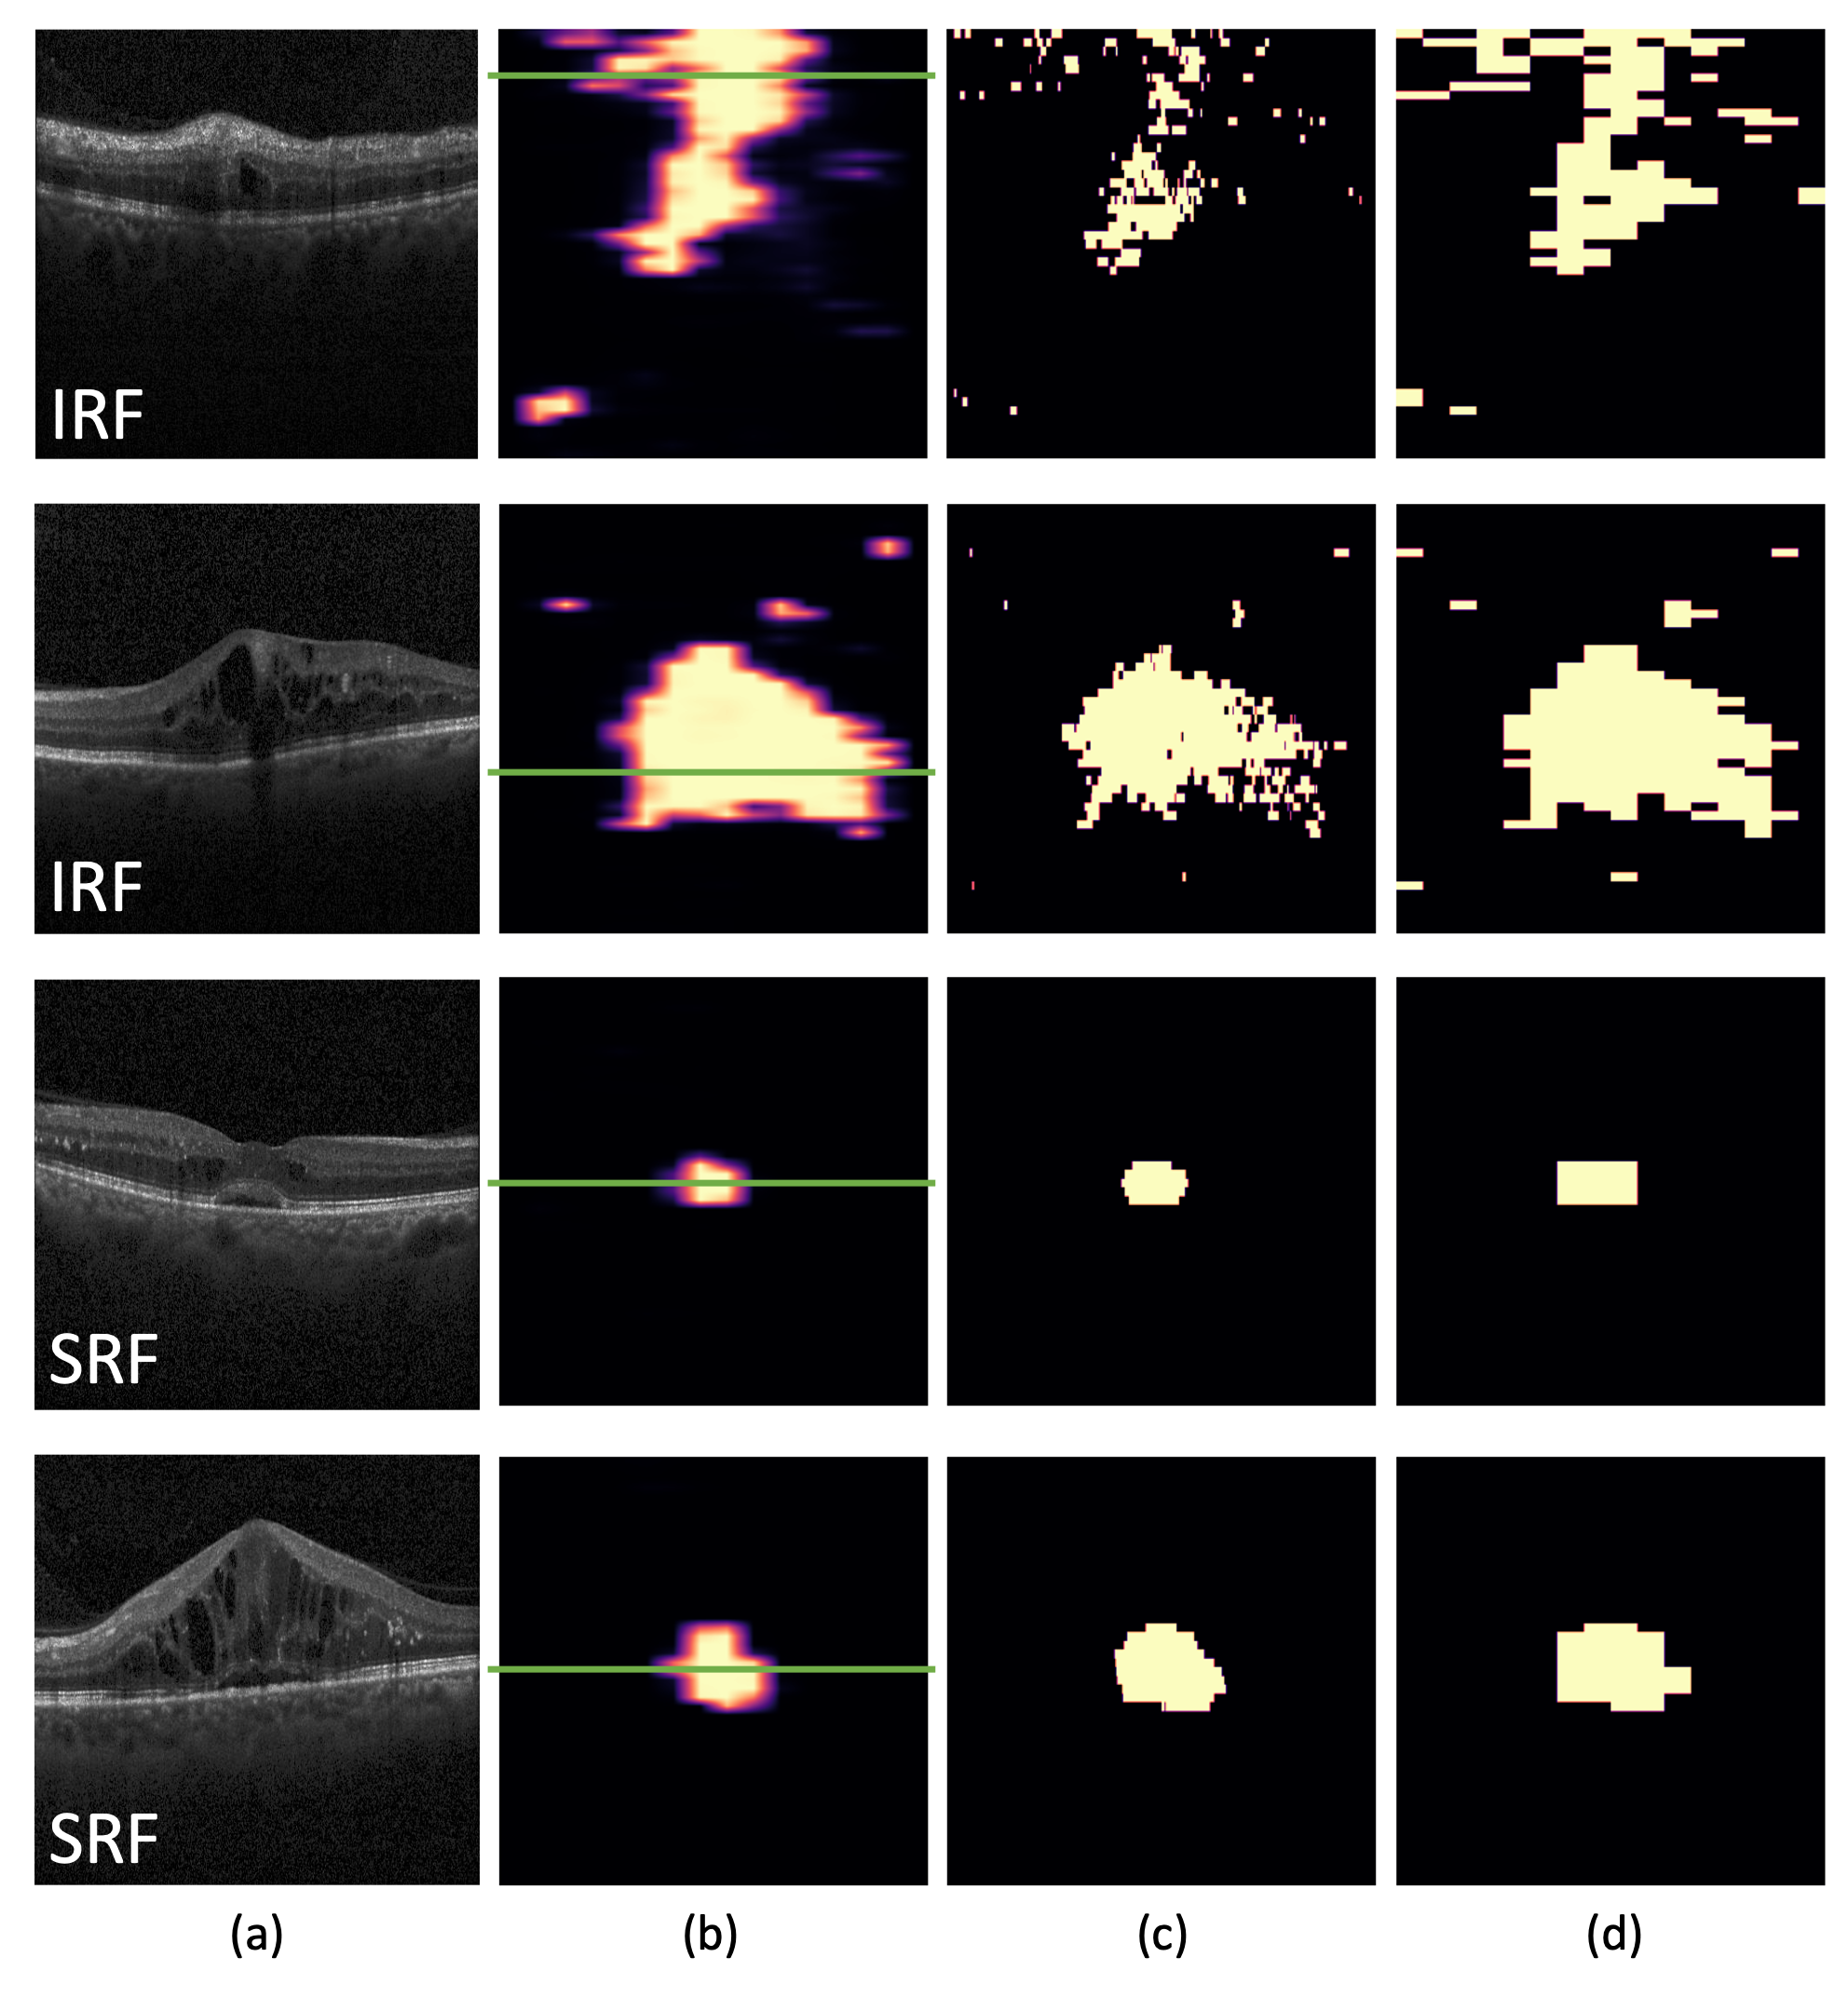
\includegraphics[width=.7\textwidth]{Figures/en_face.png}
%\caption{En-face projection results for the specified markers. (a) B-Scan at the location in green. (b) Prediction with our method. Different colors represent the uncertainty of the model. Lighter means more certain. (c) Expert pixelwise segmentation. (d) Expert segmentation converted into columns. Figure best seen in color.}
%\label{fig:en_face_qualitative}
%\end{figure}

\textfig{1}{Figures/en_face.png}{En-face projection results for the specified markers. (a) B-Scan at the location in green. (b) Prediction with our method. Different colors represent the uncertainty of the model. Lighter means more certain. (c) Expert pixelwise segmentation. (d) Expert segmentation converted into columns. Figure best seen in color.}{fig:en_face_qualitative}

To assess the clinical relevance of our method, understood as the agreement between our approach and an expert-based segmentation, we built Bland-Altman plots for SRF and IRF segmentations. In \Cref{fig:bland_altman}, we compared our prediction for the coarse \textit{en face} segmentation to the 16-column Expert in each volume. We see that four volumes fall outside one standard deviation for IRF, while only two in the case of SRF.

%\begin{figure}[htbp]
%\centering
%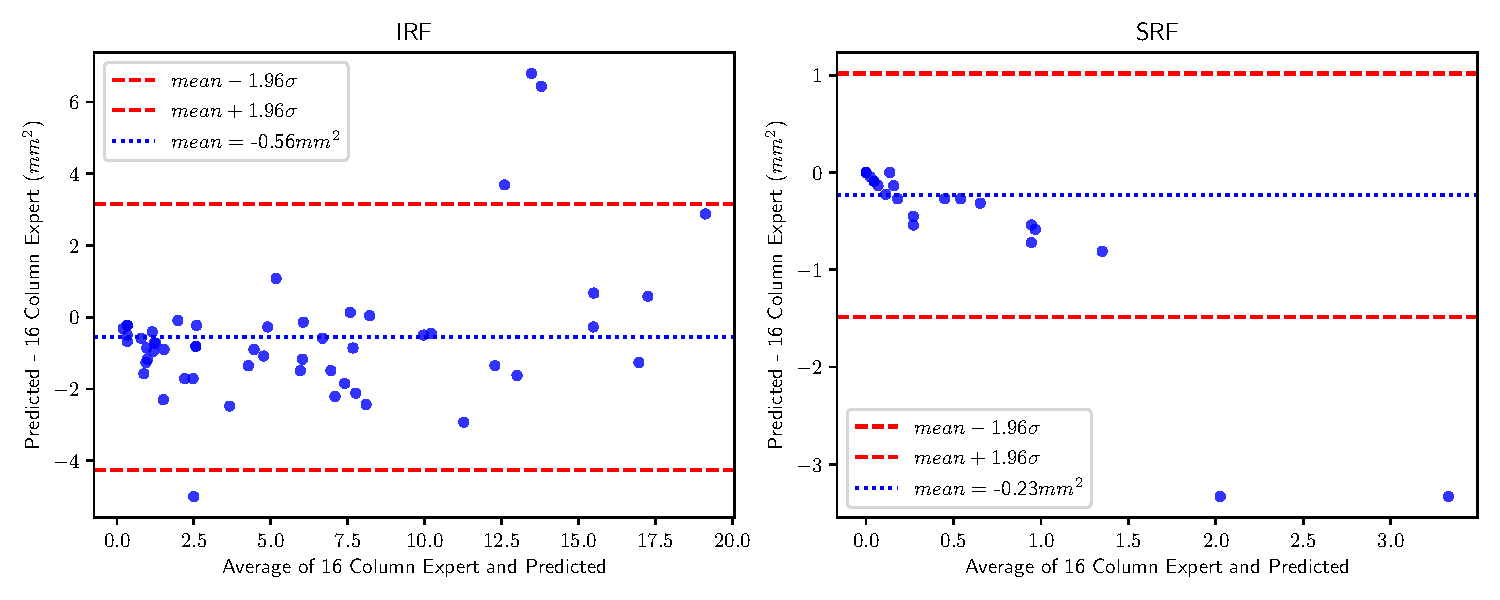
\includegraphics[width=.95\textwidth]{Figures/bland_altman.pdf}
%\caption{Bland-Altman plots for IRF and SRF}
%\label{fig:bland_altman}
%\end{figure}

\textfig[t]{1}{Figures/bland_altman.pdf}{Bland-Altman plots for IRF and SRF}{fig:bland_altman}

%\begin{figure}[htbp]
%\centering
%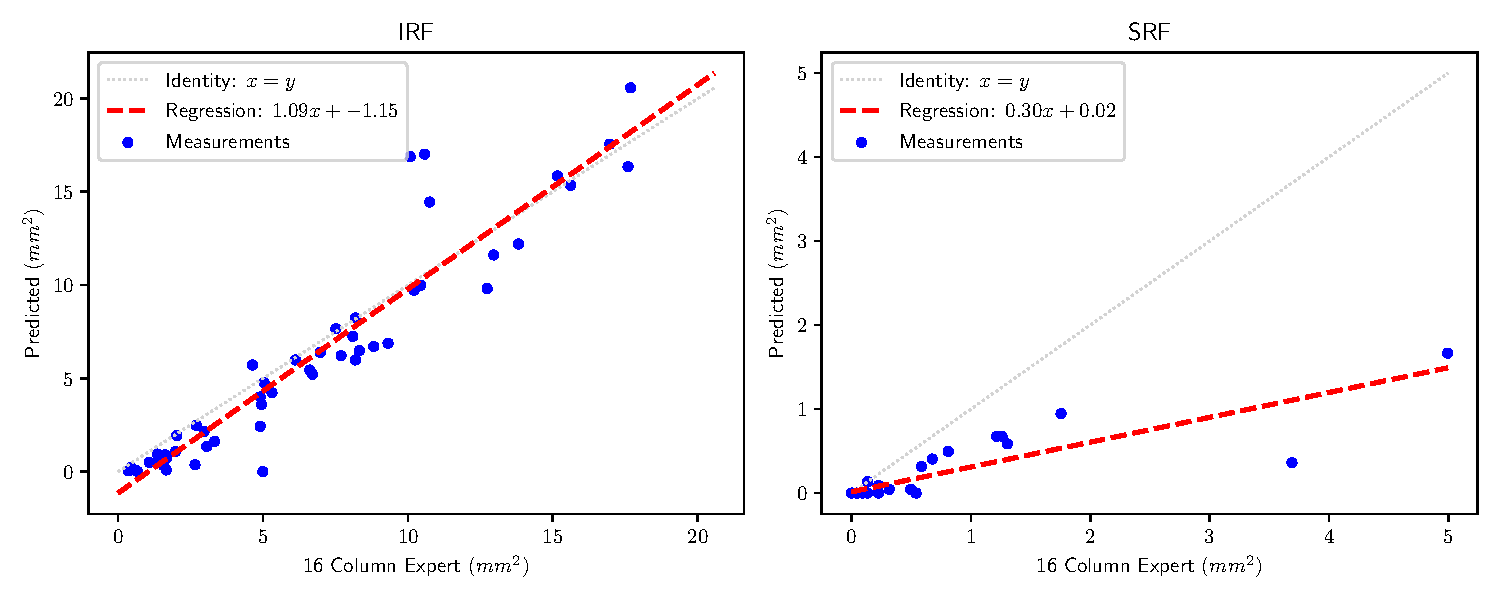
\includegraphics[width=.95\textwidth]{Figures/correlation.pdf}
%\caption{Correlation plots for IRF and SRF}
%\label{fig:correlation}
%\end{figure}

\textfig{1}{Figures/correlation.pdf}{Correlation plots for IRF and SRF}{fig:correlation}

\Cref{fig:correlation} shows correlation plots for both biomarkers. For IRF, the linear regression returns $R^2=0.895$ and a slope close to identity (1.09). On the contrary, for SRF our method achieves $R^2=0.760$ and a slope of 0.30.

\subsection{Ablation results}
We conduct an ablation study to quantify how the different loss terms in Equation 5 affect the method's performance. \Cref{tab:ablation_loc} shows the AUC ROC and AP of all predicted outputs as a function of what loss terms are included when training. The first and fourth rows, labeled with $l_1$, correspond to using the traditional Cross Entropy loss, which does not make use of any column constraint. $l_2$ and $l_3$ do impose these constraints as described in Method. On average, there is an improvement of 5.4\% ROC AUC (18.0\% AP) after the addition of column constraints, which is further increased to 7.6 and 19.1\%, respectively, with horizontal symmetry.

\begin{table*}[t]
\centering
\caption{Ablation study. We quantify the performance of our method when using only the terms \{$\ell_1$\}, \{$\ell_1$, $\ell_2$\} or \{$\ell_1$, $\ell_2$, $\ell_3$\} in our loss functions.\label{tab:ablation_loc}}
\begin{tabular}{@{}TrSSSSSS|SS@{}}
\cmidrule(l){3-10}
\multicolumn{1}{l}{} &  & \multicolumn{2}{c}{\textbf{1mm}} & \multicolumn{2}{c}{\textbf{3mm}} & \multicolumn{2}{c}{\textbf{6mm}} & \multicolumn{2}{c}{\textbf{Present}} \\ \cmidrule(l){3-10} 
\multicolumn{1}{l}{} &  & \multicolumn{1}{c}{\textbf{IRF}} & \multicolumn{1}{c}{\textbf{SRF}} & \multicolumn{1}{c}{\textbf{IRF}} & \multicolumn{1}{c}{\textbf{SRF}} & \multicolumn{1}{c}{\textbf{IRF}} & \multicolumn{1}{c|}{\textbf{SRF}} & \multicolumn{1}{c}{\textbf{IRF}} & \multicolumn{1}{c}{\textbf{SRF}} \\ \midrule
\multirow{3}{*}{\textbf{AUC}} & \multicolumn{1}{l|}{$\ell_1$} & 88.0 & 90.7 & 90.2 & 81.9 & 92.6 & \multicolumn{1}{l|}{73.7} & 96.5 & 96.2 \\
 & \multicolumn{1}{l|}{$\ell_1, \ell_2$} & 87.8 & 96.9 & 90.1 & 92.3 & 92.2 & \multicolumn{1}{l|}{91.7} & 96.5 & 95.9 \\
 & \multicolumn{1}{l|}{$\ell_1, \ell_2, \ell_3$} & \textbf{90.6} & \textbf{97.5} & \textbf{92.7} & \textbf{93.8} & \textbf{94.1} & \multicolumn{1}{l|}{\textbf{95.1}} & \textbf{97.2} & \textbf{97.7} \\ \midrule
\multirow{3}{*}{\textbf{AP}} & \multicolumn{1}{l|}{$\ell_1$} & 91.5 & 71.4 & 91.7 & 29.4 & 85.8 & \multicolumn{1}{l|}{13.8} & 96.1 & 72.3 \\
 & \multicolumn{1}{l|}{$\ell_1, \ell_2$} & 90.9 & 84.8 & 91.7 & 41.5 & 86.5 & \multicolumn{1}{l|}{\textbf{24.4}} & 96.3 & 77.1 \\
 & \multicolumn{1}{l|}{$\ell_1, \ell_2, \ell_3$} & \textbf{92.1} & \textbf{86.6} & \textbf{93.7} & \textbf{52.7} & \textbf{88.3} & \multicolumn{1}{l|}{19.1} & \textbf{96.8} & \textbf{77.9} \\ \bottomrule
\end{tabular}

\end{table*}
\section{Discussion}

The proposed method achieved satisfactory results in all ETDRS rings and studied biological markers. Our method outperforms the compared baselines for every marker and ETDRS ring, confirming our hypothesis that feature maps can be used to coarsely identify marker locations.

We note, however, that, in terms of AP, the prediction performance for SRF in the 3mm and 6mm rings is significantly lower than other reported values for all methods. As discussed in the Results section, it is unlikely to find SRF in the outer rings, leading to a lower number of occurrences of this biological marker\sidenote{As noted in \Cref{tab:results}, only 0.4\% of the slices contain SRF in the 6mm ring, as opposed to 38.4\% for IRF.}. This in turn strongly reduces the precision of the methods as soon as there are just a few false positive detections. The associated AUC ROC scores do not exhibit this behavior since they include false positive rates.

The segmentation results in \Cref{tab:segmentation_results} show that the proposed method is robust even before our post-processing mapping for coarse biomarker localization, meaning that the post-processing step is transparent to the performance of the model. 

The ablation studies in \Cref{tab:ablation_loc} suggest that not only is the architecture itself important ($\ell_1$) but so is enforcing coherence in the column outputs with the slice labels (i.e. $\ell_2$). In the case of SRF at 3mm and 6mm, this provides a significant performance increase without reducing the performances of other outputs. For SRF, AP increases by 41.2\% at 3mm and 43.4\% at 6mm, while close to no difference is seen for IRF, where the results with $\ell_1$ already outperform some of the baselines. This boost at the outer rings is highly beneficial as the presence of biological markers in these rings (especially SRF) is highly scarce, therefore making it harder to train appropriately for. In our testing dataset, acquired with a variety of eyes and patients, only 113 out of 28’322 B-Scans showed SRF in the 6mm ring. Finally, including $\ell_3$ brings modest but consistent gains when $\ell_1$ and $\ell_2$ are already used.

Compared to other methods, our model is more robust than the baselines, giving more reliable results even in hard situations where previous methods struggle. Grad-CAM is the go-to method in virtually all weakly supervised segmentation methods for OCT, which rely on a CAM-based approach with various architectures. In this line, MS-CAM~\sidecite{ma2020} proposes an architecture that leverages the activations of the different feature resolutions of the backbone and then combines them with Grad-CAM++. Segmentations are then refined using CRF on the en-face projection image. For a fair comparison with our method, which does not use C-Scan information, we implemented only the first stage. The results in \Cref{tab:results} show a performance worse than other baselines, with a strong difference in more difficult scenarios. For SRF at the 6mm ring, MS-CAM achieves 1.6 AP, compared to 19.1 with our method. We believe that CRF refinement plays a major role in MS-CAM by reducing the over-segmentation produced by the first stage. Over-segmentation leads to false positive predictions in our set-up, which reduces Average Precision.

Szeskin et al.~\sidecite{Szeskin2021} use vertical pixel-wide columns in OCT slices to classify atrophic regions. Each B-Scan is partitioned into columns and fed with contiguous slices into a convolutional neural network, which outputs a binary label. The results are projected onto the infrared imaging image and are used to identify and segment atrophy lesions. Although this work looks similar to ours, it differs in the training scheme: while we only use slice-level annotations, allowing us for independent coarse segmentation per slice; the method proposed by Szeskin et al.~\sidecite{Szeskin2021} uses per volume labeling in the form of IR image segmentation.
Schlegl et al.~\sidecite{Schlegl} focuses on voxel-wise segmentation and, while their output could be used for location as well, the method differs in intent and uses voxel-wise ground truth labels to train. Because our method uses only 2D slices and much weaker annotations, we believe it is not a comparable baseline.

Finally, the analysis of the en-face projection and segmentation results in \Cref{tab:segmentation_results}, as well as \Cref{fig:bland_altman} and \Cref{fig:correlation}, shows two aspects: 1) The outperformance of our model over the baselines does not depend on the post-processing step and 2) although both the training and inference act per B-Scan, the method is reliable and consistent when applied to all the slices in a volume. The Bland-Altman plot in Figure 8, along with the correlation plot in \Cref{fig:correlation}, show that our area predictions per volume strongly agree with the Expert segmentation in the case of IRF. For SRF, this task remains challenging, and our method tends to underestimate the en-face area, as proved by the slope of 0.30 in the linear regression and the corresponding Bland-Altman plot. However, the end goal of our method is not to have an accurate segmentation of the en-face, but it comes as a byproduct.

We demonstrated that slice-level labels are sufficient to locate biological markers in ETDRS rings for OCT scans if weak constraints are enforced on the loss function. Furthermore, we confirmed that it is possible to modify the pooling strategy of a standard convolutional network to perform coarse localization without annotations. The method has proven to be more reliable than other baselines, even in hard situations where the number of training samples is scarce, as shown in \Cref{tab:results}. The ablation experiments in \Cref{tab:ablation} demonstrate that the new terms in the loss function, especially $\ell_2$, are key to the performance of the model, producing consistent gains in all scenarios. Moreover, even if our method has only been presented with individual B-Scans during training, with no sense of complete volumes, it is capable of outputting volume-wise consistent predictions, as depicted in the segmentation and en-face projection results (\Cref{tab:segmentation_results} and \Cref{tab:en_face} respectively). Lastly, there is no constraint in the loss function with regard to the markers that can be located. Therefore, the described approach could potentially be used to locate any biological marker as long as class labels are available.

\subsection{Limitations}
Our approach has some limitations. Most notably, the granularity of the output before post-processing is constrained by the resolution of the feature maps. A more granular output would most likely improve the precision of the method. However, achieving such high-resolution feature maps collides with the main intention of classification neural networks, which are conceived to reduce the dimensionality of the inputs before the final linear layer. Another limitation comes from the variety of biological markers that have been tested. Due to labeling capacity and present pathologies in the data, only IRF and SRF were tested. Although the proposed method is agnostic to this aspect and potentially should behave equally with a larger cohort of markers, a more detailed study is required to confirm it.

\section{Conclusion}
\label{sec:tist_conclusion}

We proposed a novel self-training framework with a self-assessment strategy for pseudo-label reliability, namely ``Transformation-Invariant Self-Training'' (TI-ST). This method uses transformation-invariant highly-confident predictions in the target dataset by considering an ensemble of high-confidence predictions from transformed versions of identical inputs. We experimentally show the effectiveness of our approach against numerous existing methods across three different source-to-target segmentation tasks, and when using different model architectures. Beyond this, we show that our approach is resilient to changes in the methods hyperparameter, making it well-suited for different applications. 